\chapter{Interpretability and Case-Level Explanation}
\label{chap:explainability}

\section{Why Interpretability, and Why at Three Levels}

Chapter~\ref{chap:results} establishes that the heterogeneous graph
transformer predicts case outcomes more accurately than non-graph
references and that it does so without relying on identity shortcuts.
Those are necessary conditions for a legal-prediction model, but they
are not sufficient. A legal audience, practitioners, auditors,
reviewers, does not evaluate a prediction system purely on aggregate
accuracy; it evaluates it on whether individual predictions can be
\emph{read}, and on whether the aggregate accuracy is explained by
legally coherent structure rather than by incidental corpus
regularities.

This chapter treats the trained HGT as a \emph{frozen} object and
dissects it through three progressively finer lenses. Presenting the
analysis as a single pipeline rather than a set of unrelated tools is
deliberate: each lens answers a different question but operates on the
same artefacts, the pre- and post-GNN case embeddings, the frozen
graph, and the trained checkpoint, so the results are directly
comparable.

\begin{enumerate}
  \item \textbf{Representation-level analysis.} \emph{Does the GNN
    learn anything beyond the input features?} A probing classifier
    and t-SNE visualisation characterise the learned case embedding
    and measure the gain contributed by message passing.
  \item \textbf{Component-level analysis.} \emph{Which node and edge
    types does the model actually depend on?} Node-type zeroing,
    per-relation attention, and SHAP over the post-GNN embedding
    identify the graph components whose removal most degrades
    performance.
  \item \textbf{Case-level explanation.} \emph{For one prediction,
    \emph{why}?} A heterogeneous edge-masking explainer combined
    with LLM verbalisation produces, for a chosen test case, the
    statutes, provisions, precedents, and argument spans the frozen
    model used, and verbalises that evidence bundle into a legal
    narrative. A complementary diagnostic uses the same PGE outputs
    to read individual misclassifications: it walks each top-ranked
    node back to its training-case neighbours and reports the
    outcome-label distribution that the GNN propagated through.
\end{enumerate}

The first two levels operate globally, one model, many cases.
The third operates locally, one case at a time. The bridge between
them is the post-GNN case embedding: representation-level analysis
establishes that this embedding carries outcome-relevant structure,
component-level analysis identifies which graph signals shape it, and
case-level explanation uses the trained edge masker to ground
individual explanations in legally named evidence.

\section{Representation-Level Analysis: What Did the GNN Learn?}
\label{sec:repr_analysis}

The probing-classifier comparison in Chapter~\ref{chap:results} already
established that the 64-d post-GNN \textsc{Case} embedding outperforms
the 1036-d pre-GNN feature vector by a non-trivial margin under an
identical L2 logistic-regression head and an identical train/test
split. That number isolates the contribution of message passing from
the underlying \texttt{bge-m3} text features, but it does not say
\emph{how} the representation has been reorganised. To see the
geometry, pre- and post-GNN embeddings are projected into 2-D with
t-SNE, coloured once by legal-domain bucket and once by outcome label.

\begin{figure}[H]
  \centering
  \begin{minipage}{0.49\textwidth}
    {\footnotesize (a) Pre-GNN, coloured by domain\par}
    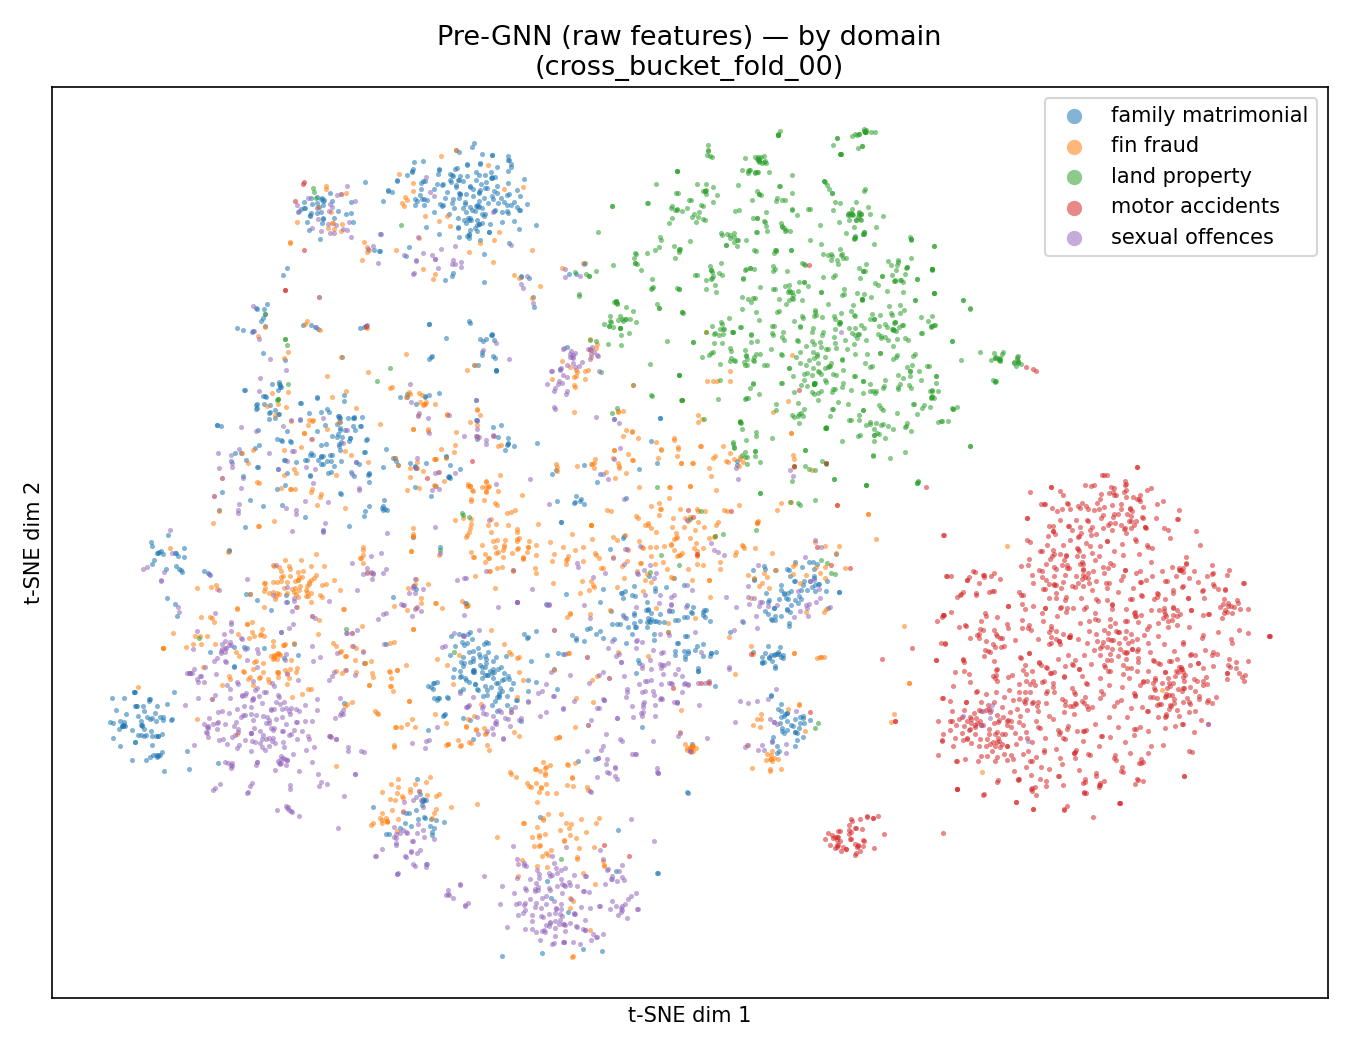
\includegraphics[width=\linewidth]{figures/explainability/tsne_pre_by_domain.png}
  \end{minipage}\hfill
  \begin{minipage}{0.49\textwidth}
    {\footnotesize (b) Post-GNN, coloured by domain\par}
    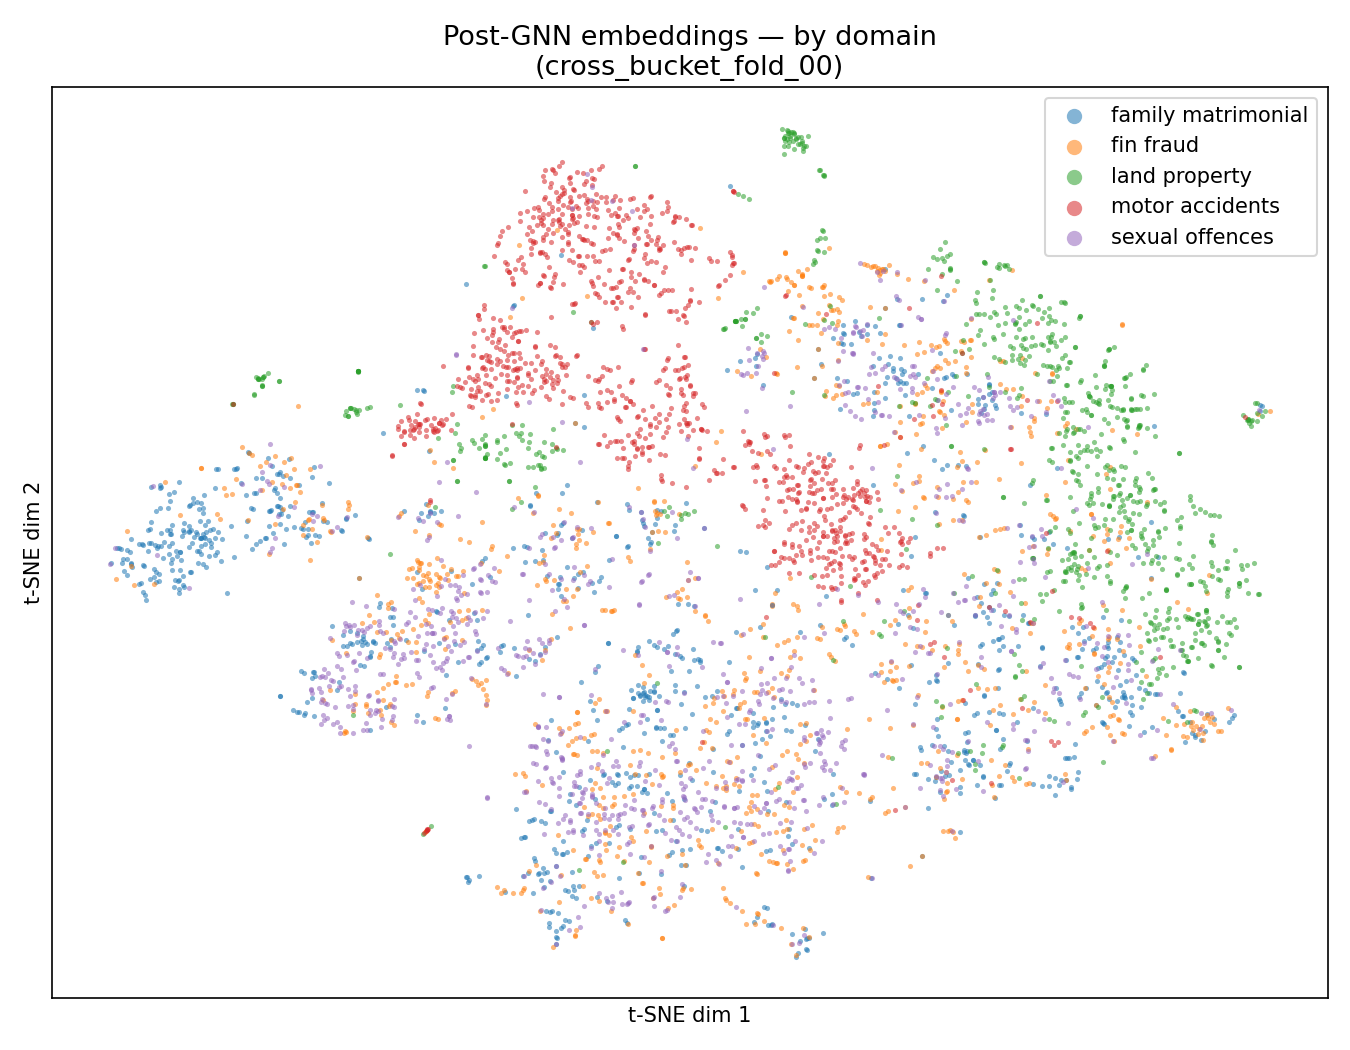
\includegraphics[width=\linewidth]{figures/explainability/tsne_post_by_domain.png}
  \end{minipage}

  \vspace{0.5em}

  \begin{minipage}{0.49\textwidth}
    {\footnotesize (c) Pre-GNN, coloured by outcome label\par}
    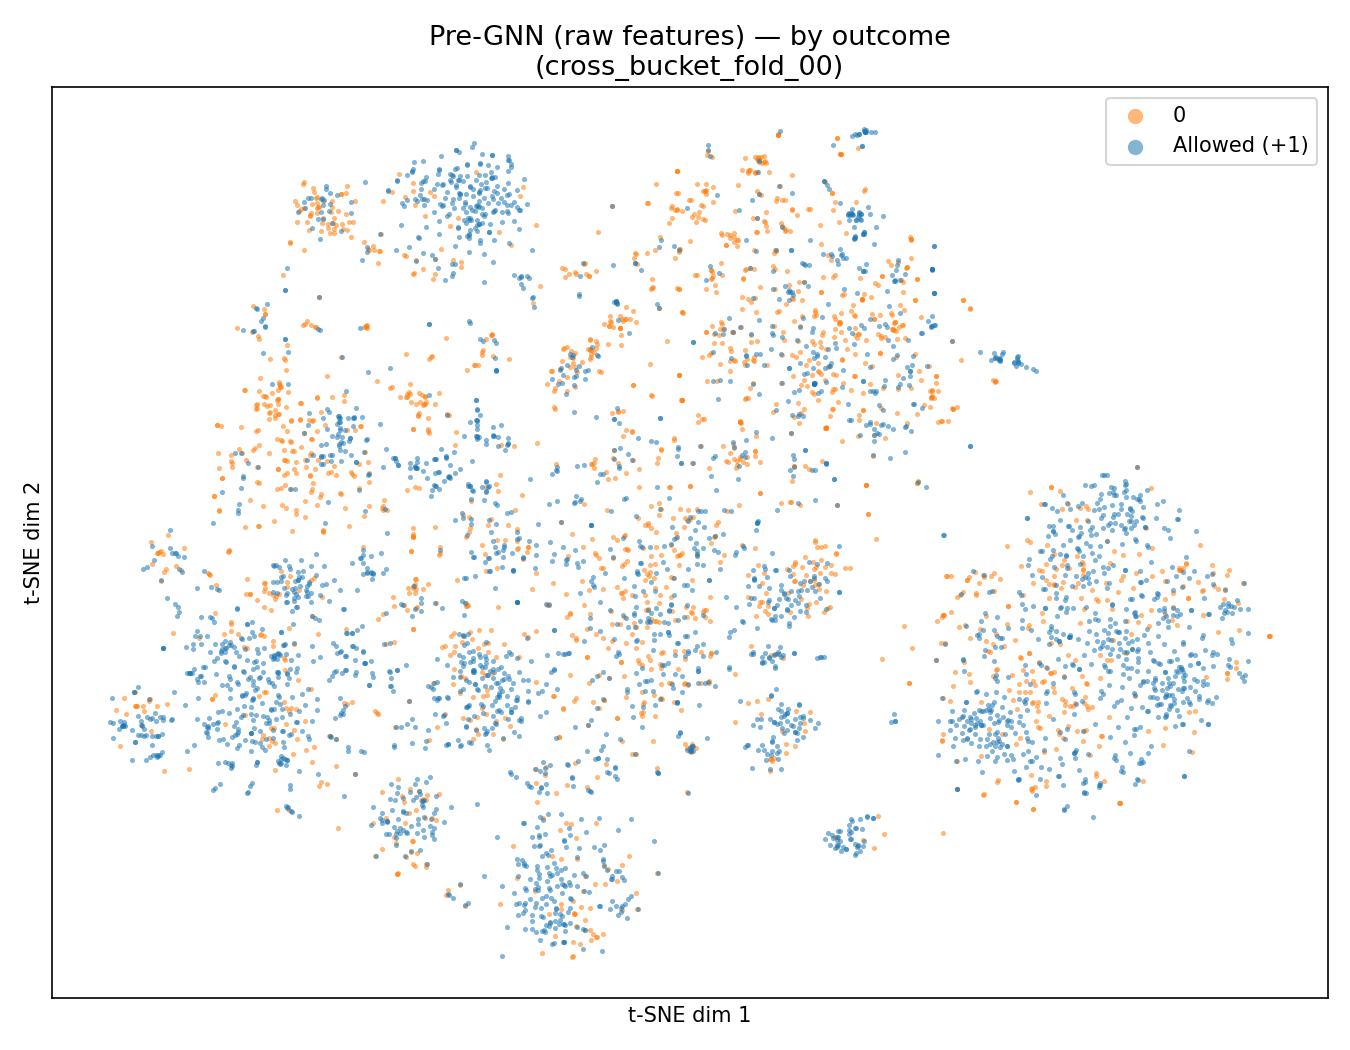
\includegraphics[width=\linewidth]{figures/explainability/tsne_pre_by_label.png}
  \end{minipage}\hfill
  \begin{minipage}{0.49\textwidth}
    {\footnotesize (d) Post-GNN, coloured by outcome label\par}
    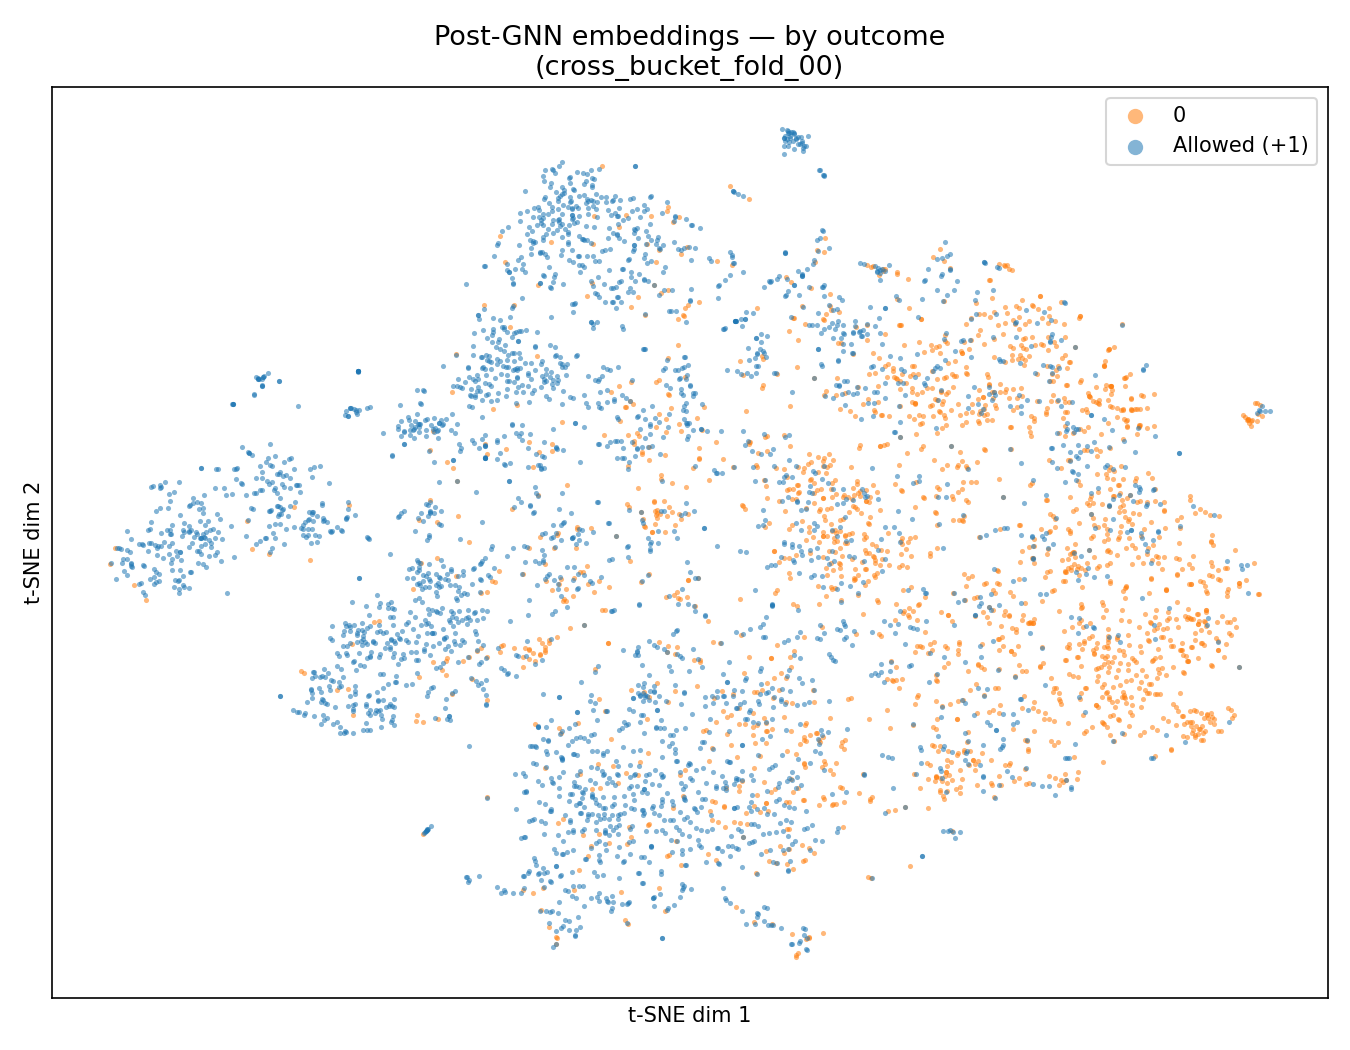
\includegraphics[width=\linewidth]{figures/explainability/tsne_post_by_label.png}
  \end{minipage}
  \caption{t-SNE projections of pre- and post-GNN case embeddings on
  fold~0 of the cross-bucket test split. Domain structure is already
  present in the pre-GNN view; label structure emerges only after
  graph propagation.}
  \label{fig:repr_tsne}
\end{figure}

The picture is consistent with the probing numbers. Pre-GNN
embeddings cluster strongly by \emph{domain}, the \texttt{bge-m3}
representation of the concatenated case text already separates the
five legal buckets, but outcome labels are mixed within each
cluster. Post-GNN embeddings preserve the domain clusters but
reorganise each cluster internally so that outcome colour becomes
visibly structured. The HGT's contribution is therefore primarily
\emph{within-domain} label geometry, not between-domain
reorganisation: message passing uses the shared hubs to sharpen
outcome separation inside each legal neighbourhood.

\section{Component-Level Analysis: Which Parts of the Graph Matter?}
\label{sec:component_analysis}

\paragraph{Problem.}
The representation-level analysis tells us the graph adds signal; it
does not tell us \emph{which} parts of the graph add it. The
heterogeneous schema has many node types and many edge types, and the
ablation table in Chapter~\ref{chap:results}
(Table~\ref{tab:cross_bucket_results}) shows that removing any one of
them has only a modest effect. That is a coarse test: it measures
\emph{re-trained} performance without a component. A complementary
question is, for the \emph{same} frozen model, which components is
the prediction \emph{using} on a case-by-case basis?

\paragraph{Three complementary probes.}
The component-level analysis uses three complementary probes: node-type
zeroing, per-relation attention with gradient saliency, and SHAP over
the post-GNN embedding. They answer different slices of the same
question, and using them together reduces the risk of any single method
producing a misleading ranking.

\paragraph{Node-type zeroing.}
For each node type in turn, all features of that type are replaced
with zeros and the frozen HGT is re-evaluated; the drop in test
accuracy is that type's importance. Across the cross-bucket baseline
the \textsc{Case} node dominates and the argument-bearing text nodes
together with \textsc{Petitioner} and \textsc{Judge} follow.
% The
% full ordering, accuracy drops, and bar-chart plot are in
% Appendix~\ref{app:node_importance}.

\paragraph{Per-relation attention and gradient saliency.}
A second probe extracts per-relation attention priors and node-type
gradient saliency, and broadly agrees with the zeroing analysis,
saliency confirms that the argument stream is the operational hinge
of the model.
% Per-relation attention heatmaps and the saliency
% ranking are in Appendix~\ref{app:attention_saliency}.

\paragraph{SHAP over the post-GNN embedding.}
The third probe computes mean absolute SHAP values for each dimension
of the 64-d post-GNN embedding under a logistic-regression probe.

\begin{figure}[H]
  \centering
  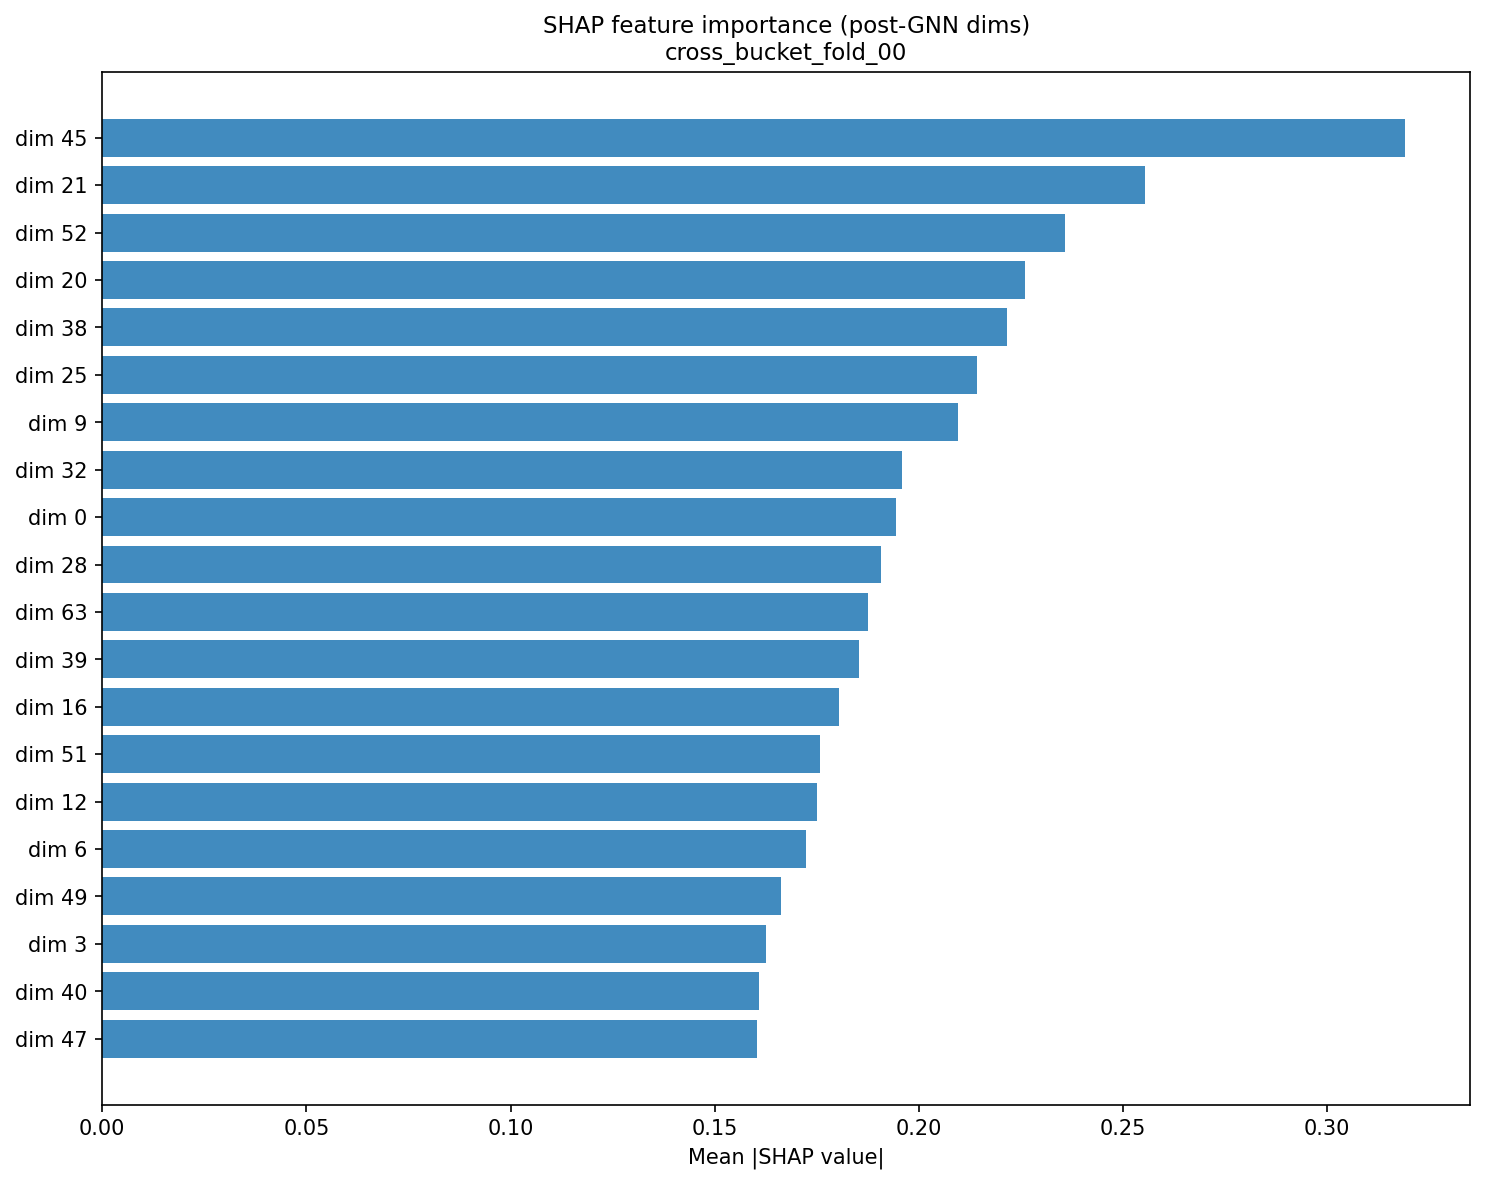
\includegraphics[width=0.78\linewidth]{figures/explainability/shap_bar.png}
  \caption{Mean absolute SHAP values per latent dimension of the
  post-GNN case embedding. The top six dimensions
  (\texttt{45, 21, 52, 20, 38, 25}) carry the largest marginal
  contribution, but no single dimension dominates.}
  \label{fig:shap_bar}
\end{figure}

No single dimension dominates: the top six dimensions each contribute
meaningfully, but the remaining $58$ dimensions still sum to a
comparable share of the total mass. A distributed embedding is
exactly what one would want from a graph-level representation,
collapse onto a small number of dimensions would be evidence of
representational bottleneck. It is worth stressing, however, that
SHAP operates on the \emph{latent} space: it identifies important
embedding \emph{dimensions}, not interpretable legal concepts. For
that reason, this probe is used as a \emph{representation diagnostic}
rather than as the final legal explanation; the case-level pipeline
of Section~\ref{sec:case_pipeline} is what produces legally named
evidence.

The global probes above answer the \emph{what} and \emph{which}
questions. What they cannot answer is the \emph{why} for any
individual prediction, why a particular case was decided the way
the model says it was, or why a confident prediction nevertheless
turned out wrong. That question requires a case-scale pipeline.

\section{Case-Level Explanation}
\label{sec:case_pipeline}

\paragraph{Problem.}
The representation- and component-level probes characterise the
model in aggregate: what the GNN learned, and which graph parts it
relies on on average. Neither speaks to a specific decision, why
\emph{this} case was predicted the way it was, or whether a confident
prediction is grounded in legally coherent evidence. Closing that gap
demands an additional, case-wise step on top of the global analyses:
for any chosen test case, surface a ranked set of \emph{legally
named} entities, statutes, provisions, precedents, and argument spans
that the frozen model actually relied on, and a natural-language
synthesis a practitioner can read.

\paragraph{Approach.}
This case-wise step is implemented as a four-phase pipeline bolted
on top of the frozen HGT checkpoint, summarised in
Table~\ref{tab:case_phases}. The bridge to the global analyses is
the post-GNN embedding: Section~\ref{sec:repr_analysis} established
that this embedding encodes outcome-relevant structure, while
Section~\ref{sec:component_analysis} identifies which graph components
shape that structure.

\begin{table}[H]
  \centering
  \footnotesize
  \begin{tabular}{@{}p{0.18\linewidth}p{0.74\linewidth}@{}}
    \toprule
    \textbf{Phase} & \textbf{Role} \\
    \midrule
    1. Inference & Run the frozen HGT once over the full graph; cache 64-d post-GNN embeddings, predicted labels, and class probabilities for every case. \\
    2. Edge masker & Train a heterogeneous edge masker against the frozen HGT, scoring how much each edge contributes to the prediction. \\
    3. Evidence & Convert edge scores into ranked statutes, provisions, precedents, and argument spans for the target case. \\
    4. Verbalisation & Pass the evidence bundle to a Mistral-Small~24B model, which writes a structured legal narrative around it. \\
    5. Misclassification diagnostic & For each top-ranked PGE node, trace it back to the training cases that connect to it via the same edge type and report the outcome-label distribution; aggregate by PGE importance to localise the neighbourhood signal driving the prediction. \\
    \bottomrule
  \end{tabular}
  \caption{Five phases of the case-level explainer. Phases 1--2 are
  one-time set-up; phases 3--5 are run per target case.}
  \label{tab:case_phases}
\end{table}

The experiments in this section use the \emph{cross-bucket} pooled
graph, fold~00 of the k-fold split (71{,}813 cases total: 51{,}705
training, 5{,}745 validation, 14{,}363 test), with the
best-performing checkpoint from Chapter~\ref{chap:results}, namely
the \texttt{party\_args\_lr\_decay} HGT (hidden dimension 64, two
message-passing layers, four attention heads, dropout $0.25$). The
pooled checkpoint is chosen so that evidence extraction can cross
domain boundaries through the shared hub structure when the graph
representation justifies it.

\subsection{Phase 1: Frozen Inference}

Phase~1 runs the frozen HGT in inference mode over the full graph
and caches, for every case node, its 64-d post-GNN embedding,
predicted outcome label, and per-class probabilities. These cached
outputs provide the prediction context used by the later explanation
steps without re-training the model.

\subsection{Phase 2: Training a Heterogeneous Edge Masker}

The textbook tool for edge attribution on GNNs is PGExplainer
\cite{luo2020parameterized}: a small MLP scores each edge, and the
top-scoring subset, fed back through the model, must preserve the
prediction. PyG's implementation is \emph{homogeneous}, it
weights messages through \texttt{edge\_weight}, which HGTConv does
not accept, since its attention is defined over typed neighbourhoods
rather than scalar-weighted messages.

\paragraph{Heterogeneous adaptation.}
The explainer keeps the PGExplainer objective but changes the mask
semantics from \emph{weighting} edges to \emph{selecting} them. A
shared MLP, fed source- and destination-node embeddings together
with a learnable relation-type embedding, emits a binary mask;
Phase~2 drops the masked edges from the typed edge dictionary and
reruns the frozen HGT on the reduced graph. The mask is relaxed to
$[0,1]$ via Gumbel-sigmoid straight-through estimation, keeping
selection discrete at inference time while remaining differentiable
during training. The objective combines three terms:

\begin{enumerate}
  \item \textbf{Prediction loss:} cross-entropy between the frozen
    HGT's predictions on the masked and full graphs, drives the
    mask to preserve the model's output.
  \item \textbf{Size regulariser:} an $\ell_1$ penalty on the
    fraction of selected edges, encourages sparse explanations.
  \item \textbf{Entropy regulariser:} an entropy penalty on the
    edge-score distribution, prevents collapse to uniform weights
    and forces hard decisions.
\end{enumerate}

Temperature is annealed from $5$ to $1$ over $30$ epochs: soft
exploration early, hard selection at convergence.

\subsection{Phase 3: From Edge Scores to Legal Evidence}

An edge-level score is not yet a legal explanation. Phase~3
translates the trained masker's output into entity-level answers.
Edge importance is computed once globally rather than per case, so
each new explanation only has to read scores off a precomputed
table. For each target case:

\begin{enumerate}
  \item Collect the $k$-hop subgraph centred on the case by
    undirected BFS, with depth matching the HGT's two
    message-passing layers, exactly the nodes whose information
    the frozen model could have propagated into the case
    representation.
  \item Restrict the precomputed edge-importance table to edges
    incident to that reachable set; the frozen HGT is not re-run.
  \item Aggregate edge scores to node importance by the
    max-incident-edge rule, and rank nodes by type to produce
    top-$N$ lists for \textsc{Statute}, \textsc{Provision},
    \textsc{Precedent}, and the four argument-node variants.
\end{enumerate}

The output is a JSON record containing predicted and true labels,
confidence scores, ranked entity lists, and the raw numerical
evidence backing each claim.

\subsection{Phase 4: LLM Translation}

A ranked list of node identifiers is machine-readable but not
human-readable: a legal explanation needs the statutes tied to the
provisions, the provisions tied to the case facts, and the case
facts tied to the argument evidence. Phase~4 passes the Phase~3
record to a Mistral-Small~24B model run locally under vLLM, prompted
to write a structured narrative covering the predicted outcome,
governing statutes, key provisions, salient precedents, argument
patterns, and a plain-language reasoning summary.

\paragraph{Role boundary.}
The LLM is not an open-ended legal reasoner: its inputs are the
evidence bundle from Phase~3 plus the pre-outcome text of the target
case (preamble and arguments). The true outcome is supplied as an
\emph{``actual outcome (for reference)''} field so that the
narrative can flag model errors instead of silently rationalising
them, but the prompt explicitly asks the LLM to explain the
\emph{predicted} label, not to re-decide the case. Evidence
selection stays with the trained explainer; verbalisation stays with
the LLM. That separation is what makes the resulting narrative
attributable to the HGT rather than to LLM priors.

\subsection{Phase 5: Training-Neighbour Misclassification Diagnostic}
\label{subsec:phase5_diagnostic}

Phases~3 and~4 surface and verbalise the evidence the model relied
on, but they do not, by themselves, explain why a particular
case-level prediction came out the way it did. Phase~5 closes that
gap by reading the PGExplainer outputs through the lens of the
training set. For each top-ranked PGE node, the diagnostic traces it
back through the graph to the set of \emph{training} cases that
connect to it via the same edge type, and computes the outcome-label
distribution of those training neighbours. A node whose training
neighbours are dominantly petitioner-winning (label~$1$) will,
through message passing, push the target case toward a winning
prediction; a node whose training neighbours are dominantly losing
($-1$) will push the other way. The per-node distributions are then
combined into a single importance-weighted aggregate, providing a
quantitative read on which neighbourhood signal in the graph drove
the prediction. The procedure is symmetric in winning and losing
labels and applies to any case, but its operational value is highest
on misclassifications, where it answers \emph{which training-set
neighbourhood the GNN propagated through} instead of leaving the
prediction as an unexplained confidence number.

\section{A Worked Example: A Case-Level Misclassification Diagnostic}
\label{sec:worked_diagnostic}

We illustrate the Phase~5 diagnostic on test case~29489 (\emph{Anjappa vs Special
Tahsildar}, 14 December 2023, land-acquisition domain). The frozen
HGT predicts \emph{petitioner wins} with probability $0.96$; the true
label is \emph{petitioner loses}. Figure~\ref{fig:case_misclass_diagnostic}
plots, for each PGE-surfaced top node, the share of its training
neighbours carrying each outcome label, ordered top-to-bottom by the
PGE importance score (\texttt{imp}). The bottom row is the
importance-weighted aggregate over all surfaced nodes.

\begin{figure}[H]
  \centering
  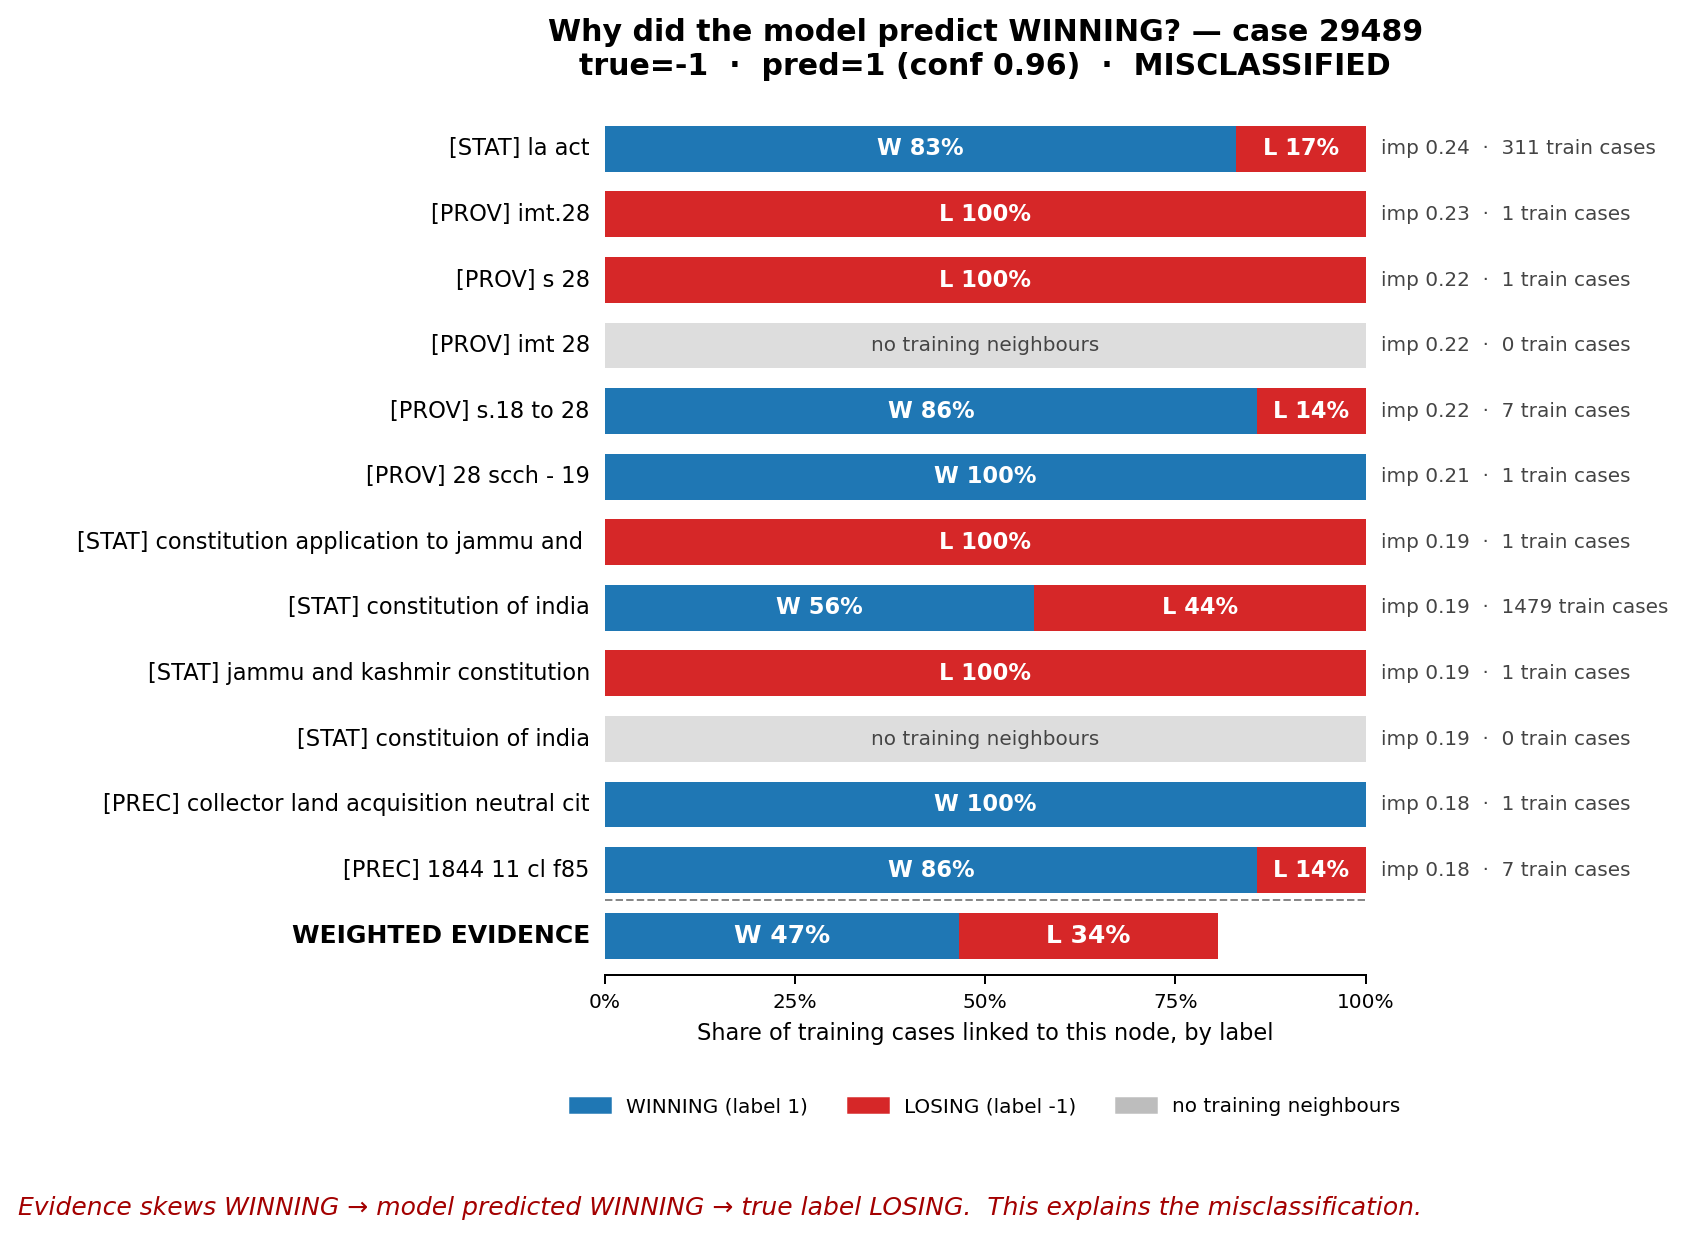
\includegraphics[width=0.95\linewidth]{figures/explainability/case_29489_misclass_diagnostic.png}
  \caption{Case-level misclassification diagnostic for case~29489
  (\emph{Anjappa vs Special Tahsildar}, 2023). Each row is a top-ranked
  PGE node; the bar shows the share of \emph{training} cases that
  connect to that node and carry each outcome label
  (W~$=$~petitioner wins, L~$=$~petitioner loses). \texttt{imp} is the
  PGE importance score for the node and is the weight used in the
  bottom row's aggregate. The cited \texttt{LA Act} statute and the
  \emph{Collector vs Mst Katiji} precedent each connect to training
  neighbourhoods that resolve overwhelmingly in favour of the
  petitioner; the importance-weighted aggregate skews the same way as
  the predicted label.}
  \label{fig:case_misclass_diagnostic}
\end{figure}

\paragraph{Reading the diagnostic.}
The most-weighted statute, the \emph{Land Acquisition Act}
($\texttt{imp}=0.24$), has $311$ training-case neighbours, of which
$83\%$ are winning. The \emph{Collector vs Mst Katiji} precedent has
$38$ training neighbours, all winning. The \emph{Constitution of
India} contributes a large but mildly W-skewed prior ($1{,}479$
neighbours, $56\%$ W). Several other surfaced provisions have only one
or two training neighbours each and contribute little to the
aggregate. Combined, the importance-weighted evidence reads
$47\%$~W~/~$34\%$~L, on the same side as the predicted label. The
diagnostic therefore localises the prediction to a specific
neighbourhood signal in the graph: the cited authorities for this case
route through training-set regions that lean petitioner-win, which is
the direction the GNN ultimately propagated.

\paragraph{Null-result reading.}
The same procedure applied to other misclassified cases sometimes
returns the opposite pattern: the per-node bars all skew toward the
true label while the model still predicts the other class. That is
informative in its own right, it indicates the prediction is not
driven by the cited statutory or precedential signal, and points to
the textual or structural part of the representation as the remaining
suspect.

\section{Summary}

The interpretability pipeline presented in this chapter provides a
coherent story for the trained HGT. At the \emph{representation}
level, a pre-GNN/post-GNN probe shows a
$+3.97$-point accuracy gain attributable to message passing, and
t-SNE confirms that the gain takes the form of within-domain outcome
reorganisation. At the \emph{component} level, node-type zeroing,
per-relation attention, and SHAP all converge on the same story: the
\textsc{Case} node dominates, but argument nodes and the immediate
participants contribute measurable graph-local signal that a plain
text classifier cannot access. At the \emph{case} level, frozen
inference, heterogeneous PGExplainer, and LLM translation produce
grounded, legally named explanations for individual predictions.

A complementary diagnostic step uses the same PGE outputs to read
individual misclassifications, tracing each top-ranked node back to its
training-case neighbours and reporting the outcome-label distribution
the GNN propagated through. This turns a case-level prediction into a
quantitative statement about which graph-local signal drove it, and
gives the post-hoc explainer operational value beyond a calibration
metric.
